\documentclass[reqno, 12pt]{amsart}
\usepackage{style}

\title[Supplementary Example]{Math 142: Supplementary Example}
\author[Blake Farman]{Blake Farman\\University of South Carolina}
\date{February 2, 2018}

\begin{document}
\maketitle

\section{A Class of Improper Integrals of Type II}
This note is concerned primarily with a geometric observation about the convergence of Improper Integrals of Type II of the form
\[\int_0^1 \frac{\dif x}{x^p}\]
stated in terms of certain Improper Integrals of Type I.
We observe that when \(p \leq 0\), the function \(1/x^p\) is defined at zero (e.g., say \(p = -2\), then \(1/x^{-2} = x^2\)), so when discussing Improper Integrals of Type II, we will assume that \(0 < p\).

  For the integral of interest, one can compute the values of \(p\) for which we have convergence directly.
  When \(p = 1\) we have
  \[\int_0^1 \frac{dx}{x} = \lim_{t \to 0^+} \int_t^1 \frac{dx}{x} = \lim_{t \to 0^+} \ln(x)\Big|_t^1 = \lim_{t \to 0^+} (0 - \ln(t)) = \lim_{t \to 0^+} -\ln(t) = \infty\]
  and for \(p \neq 1\) we have
  \[\int_0^1 \frac{dx}{x^p} = \lim_{t \to 0^+} \int_t^1 x^{-p}\dif x = \lim_{t \to 0^+} \frac{x^{1 - p}}{1 - p}\Big|_t^1 = \lim_{t \to 0^+}\left(\frac{1}{1 - p}\right)\left(1 - t^{1- p}\right).\]
  We have 
  \[\lim_{t \to 0^+} t^{1 - p} = \left\{\begin{array}{ll}0 &\text{if}\ 0 < 1 - p,\\
  \infty & \text{if}\ 1 - p < 0\end{array} \right.\]
  and so we have
  \[\int_0^1 \frac{\dif x}{x^p} = \left\{\begin{array}{ll}\frac{1}{1 - p} & \text{if}\ p < 1\\ \infty & \text{if}\ 1 \leq p.\end{array}\right.\]

  \begin{remark}
    Notice that this is almost exactly the inequality involving \(p\) that we had for the Improper Integral of Type I
    \[\int_1^\infty \frac{\dif x}{x^p}\]
    flipped the other way around.
    The remainder of this note will be devoted to a geometric explanation of \textit{why} this occurs.
  \end{remark}
  \section{Recollections on Composition Inverses}
  Now that we know for what values of \(p\) both types of integrals converge, we can make some interesting geometric observations.
  In order to do so, we first we recall a few facts about inverse functions.

  \begin{definition}
    Let \(f\) be a function.
    We say that \(f\) has a \textbf{composition inverse} if there exists a function \(f^{-1}\) such that for all \(x\) in the domain of \(f\)
    \[f^{-1} \circ f (x) = f^{-1}\left(f(x)\right) = x\]
    and
    \[f \circ f^{-1} (x) = f\left(f^{-1}(x)\right) = x.\]
    We call \(f^{-1}\) the \textbf{inverse of \(f\)}.

    When such a function exists, the domain of \(f\) is the range of \(f^{-1}\) and the range of \(f\) is the domain of \(f^{-1}\).
  \end{definition}

  An easy way to check if a function has an inverse is the following Theorem from.

  \begin{theorem}[Horizontal Line Test]
    A function \(f\) has a composition inverse if and only if any horizontal line intersects the graph of \(f\) in at most one point.
  \end{theorem}

  Geometrically, we also have a nice characterization of the graph of an inverse function.
  If \(f\) admits a composition inverse, \(f^{-1}\), then the graph of \(y = f^{-1}(x)\) is the reflection of the graph of \(y = f(x)\) across the line \(y = x\).

  \section{Some Symmetry}
  We recall that we can compute the Improper Integral of Type I
\[\int_1^\infty \frac{\dif x}{x^p}\]
as follows.
When \(p = 1\) we have
\[\int_1^\infty \frac{\dif x}{x} = \lim_{t \to \infty}\int_1^t \frac{\dif x}{x} = \lim_{t \to \infty} \ln(x)\Big|_1^t = \lim_{t \to \infty}(\ln(t) - \ln(1)) = \lim_{t \to \infty} \ln(t) = \infty\]
and when \(p \neq 1\) we have
\[\int_1^\infty \frac{\dif x}{x^p} = \lim_{t \to \infty} \int_1^t \frac{\dif x}{x^p} = \lim_{t \to \infty} \int_1^t x^{-p}\dif x = \lim_{t \to \infty} \frac{x^{1 - p}}{1 - p}\Big|_1^t = \lim_{t \to \infty} \left(-\frac{1}{p - 1}\right) (t^{1 - p} - 1).\]
We see that
\[\lim_{t \to \infty} t^{1 - p} = \left\{ \begin{array}{ll}\infty & \text{if}\ 0 < 1 - p, \\ 0 & \text{if}\ 1 - p < 0\end{array}\right.\]
  so
  \[\int_1^\infty \frac{\dif x}{x^p} = \left\{ \begin{array}{ll}\infty & \text{if}\ p < 1,\\ \frac{1}{p - 1} & \text{if}\ 1 < p.\end{array}\right.\]
  
  Now fix a number \(1 < p\), and consider the function \(f(x) = x^{-p}\) defined on \((0,\infty)\).
  One can check that any function of this type passes the horizontal line test on \((0, \infty)\) or, algebraically, we can see the function \(f^{-1}(x) = x^{-\frac{1}{p}}\) defined on \((0,\infty)\) satisfies
    \[f \circ f^{-1}(x) = f\left(x^{-\frac{1}{p}}\right) = \left(x^{-\frac{1}{p}}\right)^{-p} = x^\frac{p}{p} = x\]
  and
  \[f^{-1} \circ f(x) = f^{-1}\left(x^{-p}\right) = \left(x^{-p}\right)^{-\frac{1}{p}} = x^\frac{p}{p} = x.\]
  We make the observation that since \(1 < p\) we also have \(1/p < 1\), so we know both integrals
  \[\int_0^1 f^{-1}(x) \dif x = \int_0^1 \frac{\dif x}{x^\frac{1}{p}}\
  \text{and}\
  \int_1^\infty f(x) \dif x = \int_1^\infty \frac{\dif x}{x^p}\]
  converge.

  Moreover, we know that the graph of \(f^{-1}(x)\) is the reflection of the graph of \(f(x)\) along the line \(y = x\), so we can see from the symmetry in the graph
  \begin{center}
    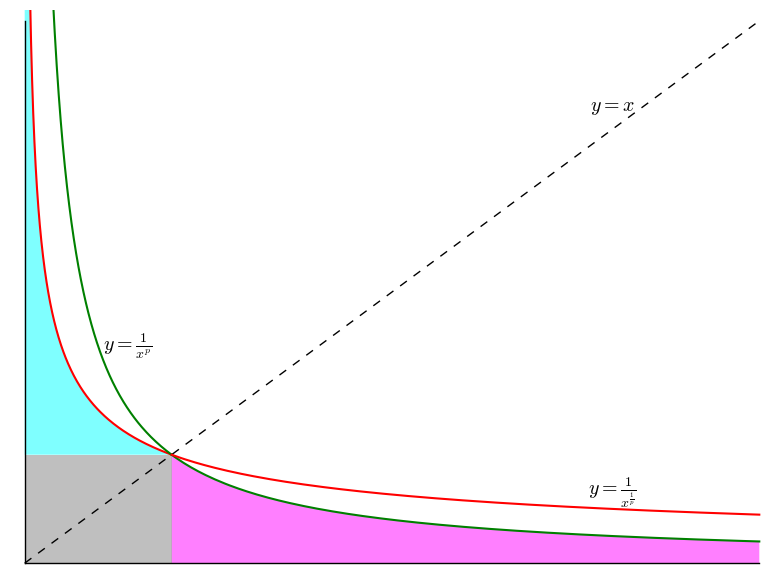
\includegraphics[scale=0.5]{symmetry}
  \end{center}
  that the blue region and the pink region have the same area, which is given by
  \[\int_1^\infty f(x)\dif x = \int_1^\infty \frac{\dif x}{x^p}.\]
  By adding together the area grey region and the area of the blue region, we should obtain 
  \[\int_0^1 f^{-1}(x) \dif x = \int_0^1 \frac{\dif x}{x^\frac{1}{p}}\]
  The grey region is just the square
  \begin{center}
    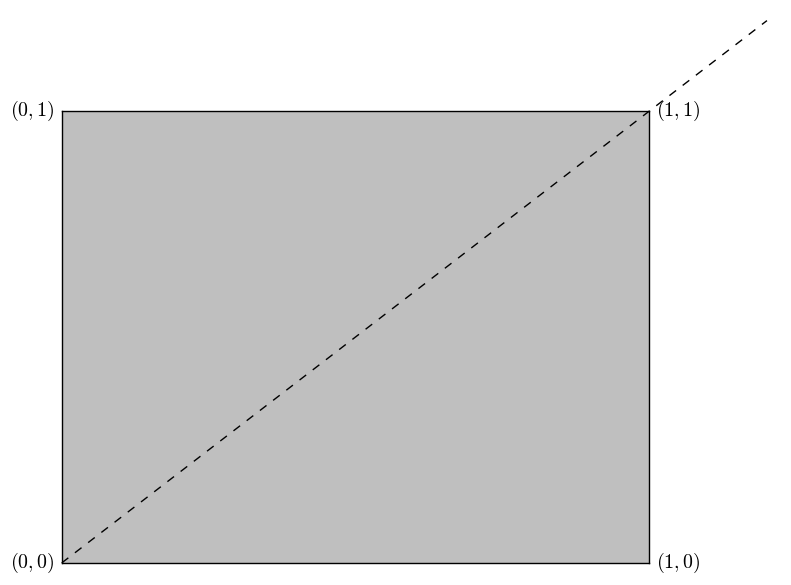
\includegraphics[scale=0.5]{square}
  \end{center}
  which has area one, so one should reasonably expect that
  \[\int_0^1 f^{-1}(x)\dif x = 1 + \int_1^\infty f(x)\dif x = 1 + \int_1^\infty \frac{\dif x}{x^p} = 1 + \frac{1}{p - 1} = \frac{p - 1 + 1}{p - 1} = \frac{p}{p - 1}.\]
  In fact, by our formula above, this is indeed the case:
  \[\int_0^1 f^{-1}(x)\dif x = \int_0^1 \frac{\dif x}{x^\frac{1}{p}} = \frac{1}{1 - \frac{1}{p}} = \frac{p}{p\left(1 - \frac{1}{p}\right)} = \frac{p}{p - 1}.\]
  Since every number in the interval \((0,1)\) can be obtained as \(1/p\) for some \(1 < p\), this gives an intuitive geometric explaination for why the Improper Integral of Type II
  %\[\int_0^1 \frac{\dif x}{x^p}\]
  converges for \(p < 1\) and diverges for \(1 \leq p\), while the Improper Integral of Type I
  %\[\int_1^\infty \frac{\dif x}{x^p}\]
  converges for \(1 < p\) and diverges for \(p \leq 1\).
\end{document}

